\documentclass{amsart} 
\usepackage{graphicx}
\graphicspath{{./}}
\usepackage[fontsize=14pt]{scrextend}
\usepackage{hyperref}
\usepackage{csvsimple}
\usepackage{epigraph}
\title{Compactness of Human Variety}
\author{Zulfikar Moinuddin Ahmed}
\date{\today}
\begin{document}
\maketitle

\section{Inspiration}

One of the most beautiful results in mathematics that I know is the Osgood-Phillips-Sarnak proof that isospectral metrics are compact for certain manifolds.  Long ago Marc Kac asked the question of whether you can hear the shape of a drum.  This is a wonderful part of mathematics.  It asks whether the Laplace spectrum of a compact manifold determines its Riemannian metric.  It was so influential for me, this result, that when I consider the Human Variety of 7.8 billion people, I am quite convinced intuitively that even in the dreams, hopes, behaviour, values, and all other aspects, there has to be some {\em compactness} that will allow us to understand the whole of it, that it is not as infinite and impossible and intractable as one might think.  Now simpleminded approaches to handling this problem would lead quickly to combinatorial intractability.  For us, getting to know even our own lover, intimate romantic soul mate is quite a difficult undertaking, because we are always balancing our evolution and sense of self and then negotiating with that of the other in that case, we are always concerned with our own autonomy and independence and then also absorbing and respecting that of the other.  It's hard work that happens in the case of intimate lovers.  And then there is always society, and society is a double edged sword.  Society offers some recognition for who we truly are one day and the next day puts us in some cage and we have to spend our days in wars to escape from the prison of society.  Life, then, is hard for us.  And life then is hard for 7.8 billion.  But that's quite alright, because all of this is from the subjective perspective, and requires experience being Zulf or being an individual.  But from a more distant perspective, such as a cold mathematical perspective that is clinically objective, compactness could still characterize the whole ball of Human Experience.  And that is what excites me at the moment.  Yes, I have had great moments of empathy for people in distant parts of the world who are not my kin and this is part of human behaviour -- that once in a while we have extraordinary empathy for people who are not our kin and yet we can feel their suffering and joy and reach out to them.  That's really nice, but quite often doing this would sabotage our own lives and so we have to be careful how we manage this.  But when we are able to see the principles behind human behaviour we can consider compactness of all of it and only then can we expect computer algorithms be able to engage with the entire human race in a sensible way.  

\section{Regularity in World Values Survey}

If you look at some of the patterns that appear in World Values Survey, if you are anything like me, be quite astounded at the regularity of percent of people who will consider one of their top motivations to make their parents proud of themselves.  Now I never even thought about it directly when I was young, because quite young I had taken the view that adults are reasonable in their way, but they were incompetent and did not really know what they were doing, and that led to me considering them with a warm feeling that they were so charming in their strange ways of seeing the world but I was doing more serious things that I won't get involved too much.  It turns out that things are quite different around the world around the exact same percentage of people consider making their parents proud to be the top motivator.  That is quite some regularity.  In fact it is such a beautiful regularity that its the sort of thing that belongs in any sort of model to characterize all human beings.  What about exceptions.  It turned out that for me making my father proud of me was a hidden motivation unknown to me that produced wild fluctuations in my life when he died in 2002.  I just did not know myself well enough!

\section{Generalized Hyperbolic Distributions}

Despite the generic name, Generalized Hyperbolic Distributions are the most important distributions in Nature.  They are much more important than Gaussian Distributions.  I will call them GHD in this note.  They are the canonical parametric distributions for skewed Gaussians, and they have been studied by Barndorff-Nielsen and his students and colleagues.  


\section{GHD Fit to Politicall uninterested People}
I took World Values Survey 2017-2020 and considered the answers across the nations of survey answers to "interested in politics". The statistics were from (very, somewhat, not very, not at all).  I added up the last two categories as a single variable, and fit the data ($N=78$) to GHD using 'fit.ghypuv' function of 'ghyp' R package. The fit is here:

\begin{verbatim}
Asymmetric Generalized Hyperbolic Distribution:

Parameters:
       lambda     alpha.bar            mu
 1.573717e+00  1.506216e-08  7.134881e+01                
       sigma         gamma 
 6.751444e+00 -1.551440e+01 

Call:
fit.ghypuv(data = polint)

Optimization information:
log-Likelihood:                -300.7405 
AIC:                           611.481 
\end{verbatim}
I could attempt to put the log-likelihood value and AIC in context, but they are quite good.  

I will show you the histogram.

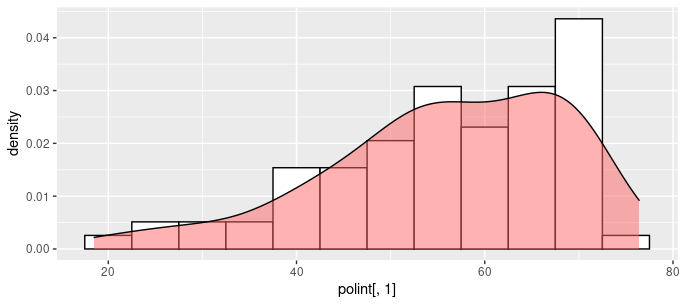
\includegraphics[scale=0.6]{unpolitical.png}

The density estimate does not show the right tail but this is quite close to a unimodal skewed Gaussian and I do not consider the deviation to be anything but noise.  This is quite a great discovery to be able to consider parametric distributions for many unlikely Human Nature variables.  

\section{Benefits}

Human Nature across all human beings is a priori intractably complex.  Taking the analogy from classical thermodynamics, we can consider thermodynamic variables such as temperature.  While the idea is attractive, there is no a priori guarantee that there will be any regularity in the distributions of any variable of interest across the global population.  We showed above that measurement data has regularity empirically.  However the regularity is far from Gaussian, and GHD fit well here.

In the most optimistic scenario all interesting variobles will have GHD distribution which is infinitely divisible and Levy, which then allows interesting mthematical theory in the quantitative side and allows us Social Science of Human Nature with GHD as primitives.

\section{One Possible Compactness Principle}

I make a nontrivial assumption that any univariate functional of a human being on Earth leads to a smooth unimodal distribution.  I don't care if there are exception because those could be decomposed, so every 'important' functional.  Then we assume $N>>1000$ is some large number of measurements of various things that have a real value attached to it.  Then we assume that for the purposes of any scientific or application interest, elements of $\mathbf{R}^N$ characterize all human beings.  Then a Generalized Hyperbolic Distribution on $\mathbf{R}^N$ is the Human Nature model.  Then any person $h$ in Humans has a functional $F(h)$ in $\mathbf{R}^N$ and this $F(h)$ is a sample for the Generalized Hyperbolic Distribution.  This could be a good Human Nature model.  All correlations are absorbed in the fitting.  Certainly this will have superior predictive power over the current technology because today correlations are considered for qualitative deductions.  I am just quite excited to see continuous skewed Gaussians in measured data so this is the optimistic approach to Human Nature.

\section{GHD For Feeling Close To The World}

An indirect measure of the spiritual expansiveness of a people is whether they feel close to the world.  We have a GHD fit for the percent in a country that feels close to the world.

\begin{verbatim}
> summary(fit.worldclose)
Asymmetric Generalized Hyperbolic Distribution:

Parameters:
       lambda     alpha.bar            mu
   -14.766895 495164.067424     45.304490
       sigma        gamma
    15.949497      3.145018 

Call:
fit.ghypuv(data = worldclose)

Optimization information:
log-Likelihood:                -330.8918 
AIC:                           671.7837 
\end{verbatim}

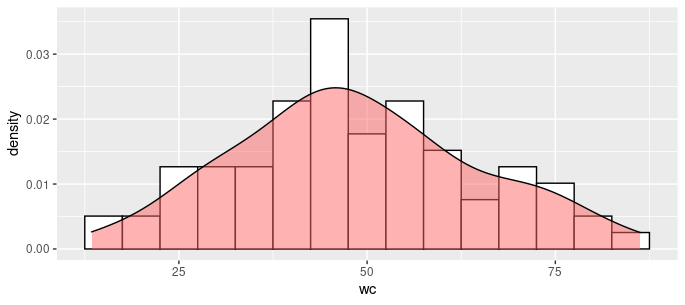
\includegraphics[scale=0.7]{worldclose.png}

I want to point out that the fit is good with nontrivial gamma, lambda, alphabar, the parameters giving non-Gaussianity.  Once again there is no theory that would predict any parametric distribution for such a non-trivial metric.


I also fit the percentage of those who feel not at all close to the world.   

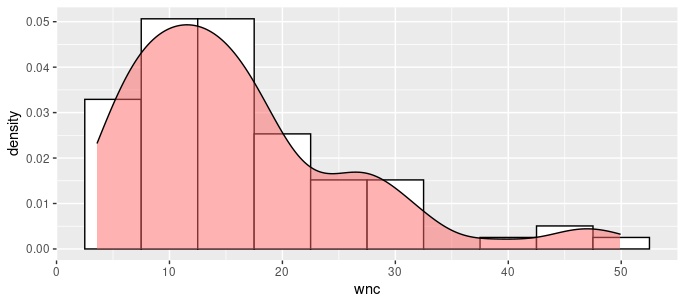
\includegraphics[scale=0.7]{worldnotclose.png}

Suppose you sampled a person randomly from the human race, and you ask "do you feel close to the world" assuming countries had equal population, their {\em probability} of answering "not at all" is in this histogram.  This is elementary.  It is a stunning surprise that any accuracy is obtained by using a {\em parametric GHD} for a scientific model of this, since there might be a million factors that determine this a priori.

\begin{verbatim}
> summary(fit.wnc)
Warning: fitting procedure did not converge!

Asymmetric Generalized Hyperbolic Distribution:

Parameters:
   lambda alpha.bar        mu
 1.333624  1.347152  1.514230 
sigma        gamma 
  1.187686   14.882737 

Call:
fit.ghypuv(data = worldclose$wnc)

Optimization information:
log-Likelihood:                -278.1262 
AIC:                           566.2524 
\end{verbatim}


\end{document}